\section{Anhang}

\subsection{Laborbuch}
\begin{minipage}{\textwidth}
	\centering
	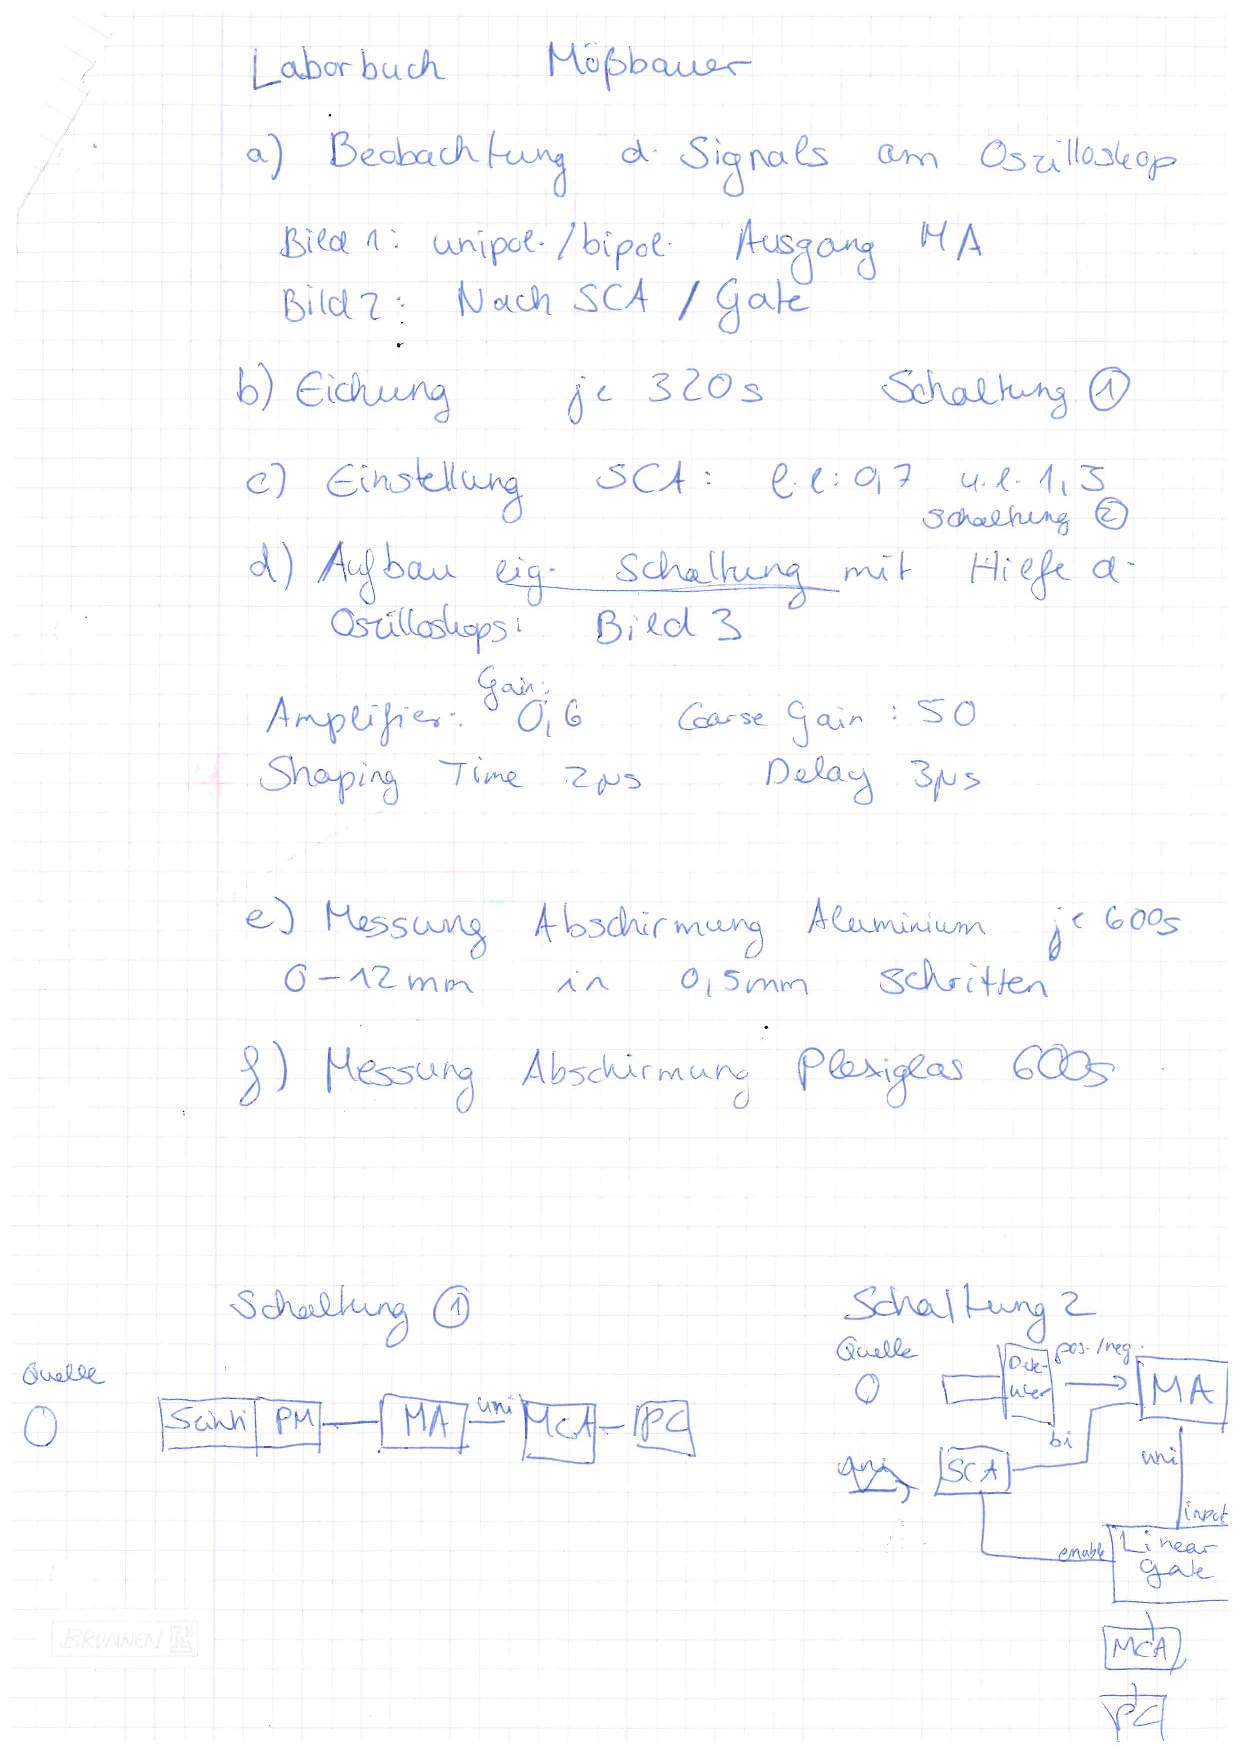
\includegraphics[width=0.9\textwidth]{../figures/laborbuch1.pdf}
\end{minipage}

\begin{minipage}{\textwidth}
	\centering
	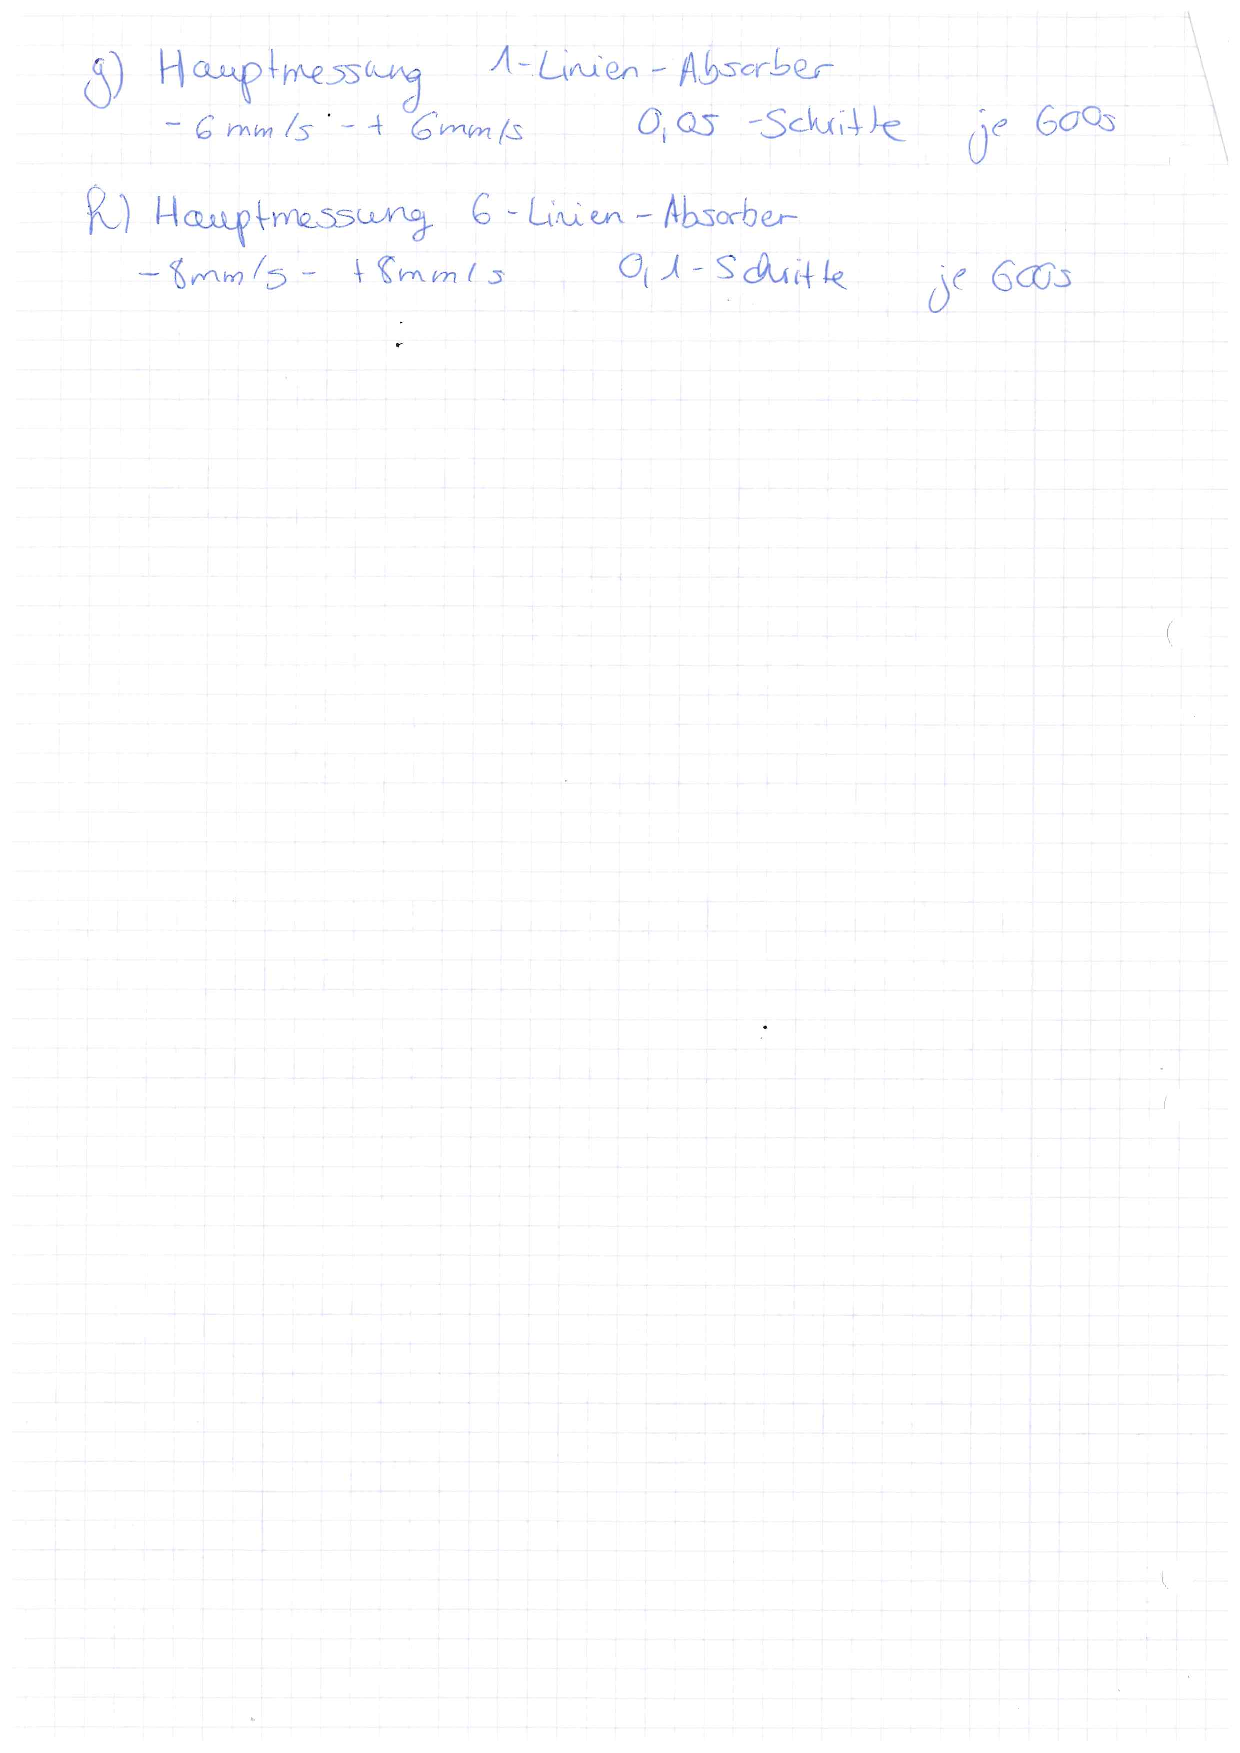
\includegraphics[width=0.9\textwidth]{../figures/laborbuch2.pdf}
\end{minipage}

\subsection{Spektren}
\label{spektren}

\subsection{Sourcecode}
\label{code}
\subsubsection*{Eichung.R}\label{Energieeichung}
\lstinputlisting[language=R]{../scripts/Eichung.R}

\subsubsection*{LinFitEichung.R}\label{LinFitEichung}
\lstinputlisting[language=R]{../scripts/LinFitEichung.R}

\subsubsection*{Compton-Untergrund.R}\label{Compton-Untergrund}
\lstinputlisting[language=R]{../scripts/aluminium.R}

\subsubsection*{Plexiglas.R}\label{Plexi}
\lstinputlisting[language=R]{../scripts/plexiglas.R}

\subsubsection*{Absorberdicke.R}\label{Absorberdicke}
\lstinputlisting[language=R]{../scripts/absorberdicke.R}

\subsubsection*{Debye-Waller.R}\label{debye}
\lstinputlisting[language=R]{../scripts/debyewaller.R}

\subsubsection*{Einlinien.R}\label{einlinien1}
\lstinputlisting[language=R]{../scripts/einlinien.R}

\subsubsection*{Sechslinien.R}\label{sechslinien}
\lstinputlisting[language=R]{../scripts/sechslinien.R}

\subsubsection*{Expfit.R}\label{exp}
\lstinputlisting[language=R]{../scripts/expfit.R}

\subsubsection*{functions.R}\label{functions}
\lstinputlisting[language=R]{../scripts/functions.R}

\subsubsection*{Gausfit.R}\label{gaus}
\lstinputlisting[language=R]{../scripts/gausfit1.R}

\subsubsection*{Lorentzfit.R}\label{lorentzfit}
\lstinputlisting[language=R]{../scripts/lorentzfit.R}

\subsubsection*{ReadFiles.R}\label{Read}
\lstinputlisting[language=R]{../scripts/readFiles.R}

\subsubsection*{Supergaus.R}\label{supergaus}
\lstinputlisting[language=R]{../scripts/supergaus.R}

\subsubsection*{Voigtfit.R}\label{voigtfit}
\lstinputlisting[language=R]{../scripts/voigtfit.R}

